% ===========================================================================
% Ajuster des modèles
% Traduit et adapté de :
%   https://www.bootstrapworld.org/materials/fall2026/en-us/lessons/fitting-models/
% Adapté au contexte français (colonnes et données en français)
% Licence : Creative Commons 4.0 Unported (Bootstrap Community)
% ===========================================================================

\documentclass[12pt,a4paper]{article}

% ---------- Packages ----------
\usepackage[utf8]{inputenc}
\usepackage[T1]{fontenc}
\usepackage{libertine}
\usepackage{microtype}
\usepackage[french]{babel}
\usepackage{graphicx}
\usepackage{float}
\usepackage{hyperref}
\usepackage{geometry}
\usepackage{enumitem}
\usepackage{tabularx}
\usepackage{xcolor}
\usepackage{colortbl}
\usepackage[raster]{tcolorbox}
\usepackage{booktabs}
\usepackage{fancyhdr}
\usepackage{titlesec}
\usepackage{amsmath}
\usepackage{amssymb}
\usepackage{listings}
\usepackage{tikz}
\usetikzlibrary{arrows.meta, positioning, calc, datavisualization}

% ---------- Mise en page ----------
\geometry{margin=2.5cm, headheight=15pt, footskip=30pt}
\fancyhf{}
\fancyhead[L]{\textbf{Ajuster des modèles}}
\fancyhead[R]{\thepage}
\fancyfoot[C]{Bootstrap Community — CC BY 4.0}
\renewcommand{\headrulewidth}{0.4pt}
\pagestyle{fancy}

% ---------- Couleurs ----------
\definecolor{bsblue}{RGB}{41,128,185}
\definecolor{bsgreen}{RGB}{39,174,96}
\definecolor{bsorange}{RGB}{230,126,34}
\definecolor{bsgray}{RGB}{149,165,166}
\definecolor{codebg}{RGB}{245,247,250}
\definecolor{modelline}{RGB}{41,128,185}
\definecolor{datadot}{RGB}{192,57,43}

% ---------- Styles de sections ----------
\titleformat{\section}[hang]{\Huge\bfseries\color{bsblue}}{}{0pt}{}[\vspace{-0.5em}\rule{\textwidth}{2pt}]
\titleformat{\subsection}[hang]{\Large\bfseries\color{bsblue!80!black}}{}{0pt}{}
\titleformat{\subsubsection}[hang]{\large\bfseries\color{bsgreen!60!black}}{}{0pt}{}

% ---------- Environnements personnalisés ----------
\newtcolorbox{overviewbox}{
  colback=bsblue!5!white, colframe=bsblue!60!white,
  fonttitle=\bfseries, title=Objectif de la section,
  left=1em, right=1em, top=0.5em, bottom=0.5em
}
\newtcolorbox{activitybox}{
  colback=bsgreen!5!white, colframe=bsgreen!60!white,
  fonttitle=\bfseries, title=Activité,
  left=1em, right=1em, top=0.5em, bottom=0.5em
}
\newtcolorbox{thinkbox}{
  colback=bsorange!5!white, colframe=bsorange!60!white,
  fonttitle=\bfseries, title=Réflexion,
  left=1em, right=1em, top=0.5em, bottom=0.5em
}
\newtcolorbox{keypointbox}{
  colback=bsgray!10!white, colframe=bsgray!50!white,
  fonttitle=\bfseries, title=Point clé,
  left=1em, right=1em, top=0.5em, bottom=0.5em
}
\newtcolorbox{instructornotes}{
  colback=yellow!10!white, colframe=yellow!80!black,
  fonttitle=\bfseries, title=Notes pour l'enseignant·e,
  left=1em, right=1em, top=0.5em, bottom=0.5em
}
\newtcolorbox{codebox}{
  colback=codebg, colframe=bsgray!40,
  fonttitle=\bfseries, title=Code Pyret,
  left=1em, right=1em, top=0.5em, bottom=0.5em
}
\newtcolorbox{contractbox}{
  colback=bsblue!3!white, colframe=bsblue!40!white,
  left=1em, right=1em, top=0.6em, bottom=0.6em
}

% ---------- Style listings pour Pyret ----------
\lstdefinelanguage{Pyret}{
  keywords={use,context,url-file,and,or,not,if,else,for,fun,data,sharing,include,import,as,where,let,rec,is,=,true,false,load-table,source,end,Row,String,Number,Boolean,Table,Image,scatter-plot,fit-model,dot-plot,box-plot},
  sensitive=true,
  comment=[l]{\#},
  morestring=[b]",
  morestring=[b]',
}
\lstset{
  language=Pyret,
  basicstyle=\ttfamily\small,
  commentstyle=\color{bsgreen!70!black}\itshape,
  keywordstyle=\color{bsblue}\bfseries,
  stringstyle=\color{bsorange},
  backgroundcolor=\color{codebg},
  frame=single,
  framesep=5pt,
  rulecolor=\color{bsgray!40},
  breaklines=true,
  breakatwhitespace=false,
  showstringspaces=false,
  aboveskip=0.8em,
  belowskip=0.8em,
}

% ---------- Commandes pratiques ----------
\newcommand{\img}[3]{%
  \begin{figure}[H]
    \centering
    \includegraphics[#2]{#1}
    \caption{#3}
    \label{fig:#1}
  \end{figure}
}
\newcommand{\contrat}[1]{%
  \begin{contractbox}
    \ttfamily #1
  \end{contractbox}
}

% ---------- Informations du document ----------
\title{%
  \vspace{-2cm}
  {\Huge\bfseries Ajuster des modèles}\\[0.5em]
  {\large Droite de régression, résidus et valeur~$S$}\\[1em]
  {\normalsize Traduit et adapté depuis \href{https://www.bootstrapworld.org/materials/fall2026/en-us/lessons/fitting-models/}{Bootstrap World} (Fall 2026)}\\
  {\normalsize Adapté au contexte francophone — colonnes et données en français}\\[0.5em]
  {\normalsize Licence Creative Commons 4.0 International}
}
\date{}
\author{}

\begin{document}

\maketitle
\thispagestyle{empty}

\vspace{2cm}
\begin{center}
  \textit{Ces supports ont été développés en partie grâce au soutien de la National Science Foundation\\
  (bourses 1042210, 1535276, 1648684, 1738598, 2031479 et 1501927).}
\end{center}

\newpage
\tableofcontents
\newpage

% ===========================================================================
% SECTION 1 : VOIR DES MOTIFS, CONSTRUIRE DES MODÈLES
% ===========================================================================
\section{Voir des motifs, construire des modèles}

\begin{overviewbox}
  Les élèves apprennent que les motifs qu'ils voient intuitivement dans un nuage de points représentent une \emph{relation} entre les variables explicative et de réponse, appelée un \textbf{modèle}. Ils comparent deux modèles pour un jeu de données simple et réfléchissent à la façon de mesurer lequel s'ajuste le mieux.
\end{overviewbox}

% ---------- Launch ----------
\subsection{Lancement}

\begin{keypointbox}
Pyret possède une fonction pour tracer des nuages de points, qui prend \emph{quatre} arguments dans son Domaine~:
\begin{enumerate}
  \item La table contenant toutes les données.
  \item Le nom de la colonne à utiliser pour les étiquettes.
  \item Le nom de la colonne à utiliser pour les abscisses ($x$).
  \item Le nom de la colonne à utiliser pour les ordonnées ($y$).
\end{enumerate}

\contrat{\# scatter-plot :: (Table table, String etiquettes, String xs, String ys) -> Image}
\end{keypointbox}

\begin{activitybox}
  Regardons des données sur des lézards provenant d'un refuge pour animaux.

  \begin{itemize}
    \item Ouvrez le fichier \textbf{Échantillon de Lézards} (\texttt{Echantillon\allowbreak-Lezards\allowbreak-Starter.arr}) et cliquez sur «~Run~».
    \item Ce fichier définit la table \texttt{lizard\allowbreak-sample} et deux fonctions nommées \texttt{cy} et \texttt{jo}.
    \item Pouvez-vous trouver où \texttt{lizard-sample}, \texttt{cy} et \texttt{jo} sont définis~?
    \item Tapez \texttt{lizard-sample} dans la Zone d'Interactions. Quelles colonnes contient cette table~?
  \end{itemize}

  Faites un nuage de points («~scatter plot~») en utilisant les colonnes suivantes~:
  \begin{itemize}
    \item étiquettes — le \texttt{nom} du lézard
    \item variable explicative (axe $x$) — le \texttt{poids} en livres
    \item variable de réponse (axe $y$) — les \texttt{semaines} avant adoption
  \end{itemize}

  \begin{lstlisting}
scatter-plot(lizard-sample, "nom", "poids", "semaines")
  \end{lstlisting}
\end{activitybox}

\begin{center}
  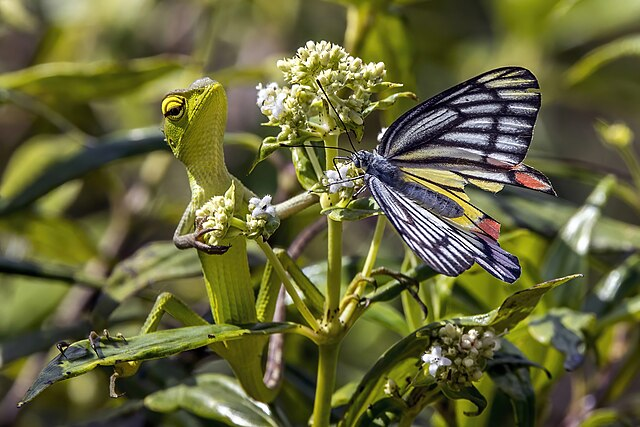
\includegraphics[width=0.28\textwidth]{images/63c8c119038f4974.png}\hfill
  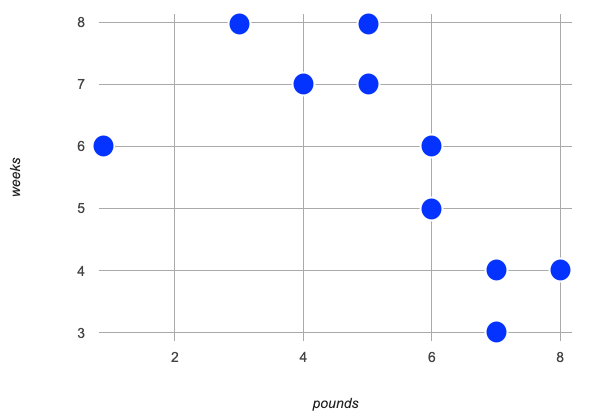
\includegraphics[width=0.50\textwidth]{images/e45941932f3c05df.png}\hfill
  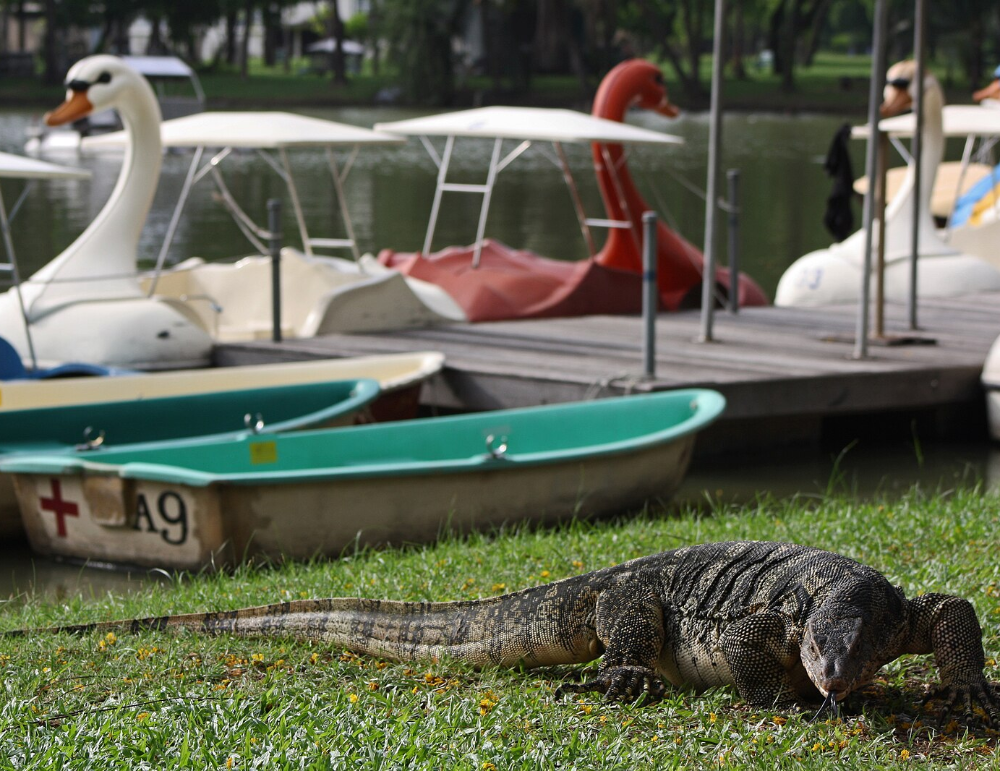
\includegraphics[width=0.18\textwidth]{images/c9b184a5f1ff0c87.png}
\end{center}
\begin{center}
\small\emph{De gauche à droite~: un petit lézard sur une fleur~; le nuage de points \texttt{poids} vs.\ \texttt{semaines}~; un grand lézard monitor près d'un bateau.}
\end{center}

\begin{thinkbox}
  \begin{itemize}
    \item \textbf{Voyez-vous un motif ici, qui relie \texttt{semaines} à \texttt{poids}~?} Si oui, comment le décririez-vous~?
    \begin{itemize}
      \item Les réponses varient mais peuvent inclure~: «~Le nombre de semaines avant adoption diminue généralement à mesure que les lézards sont plus lourds~» ou «~Les points semblent se regrouper autour d'une ligne diagonale avec une pente négative~».
    \end{itemize}
    \item \textbf{Si un nouveau lézard pesant 2~livres apparaissait, combien de temps prédiriez-vous qu'il faudrait pour qu'il soit adopté~?}
    \begin{itemize}
      \item probablement entre 7 et 10~semaines~; certainement surprenant s'il fallait moins de 6~semaines.
    \end{itemize}
    \item \textbf{Comment avez-vous fait votre prédiction~?}
    \begin{itemize}
      \item J'ai imaginé une ligne.
      \item J'ai imaginé un large pinceau qui remonte les points en partant de la droite jusqu'à arriver à 2.
      \item J'ai réfléchi au point qui pourrait venir entre $(1,6)$ et $(3,8)$, soit $(2,7)$, puis j'ai ajusté ce point vers le haut en fonction des autres points.
    \end{itemize}
  \end{itemize}
\end{thinkbox}

\begin{instructornotes}
  Conseil pédagogique~: projetez le nuage de points au tableau et demandez à des élèves de venir pointer leurs motifs du doigt.
\end{instructornotes}

\begin{activitybox}
  Tournez-vous vers la première section de \emph{Comment pourrions-nous mesurer si un modèle est un bon ajustement~? (Lézards)} et utilisez une règle pour tracer une ligne qui résume la tendance que vous voyez dans les données.

  Réfléchissez à la façon dont vous décririez cette ligne~:
  \begin{itemize}
    \item Pouvez-vous nommer deux points par lesquels elle passerait~?
    \item Pouvez-vous identifier sa pente~?
    \item Où imaginez-vous qu'elle croise l'axe des ordonnées~?
  \end{itemize}
\end{activitybox}

\begin{keypointbox}
  \textbf{Données = Modèle + Erreur}

  En traçant une ligne à travers notre nuage de points, nous définissons un \textbf{modèle}~: un résumé de la relation entre deux variables dans un jeu de données. Ce modèle nous permet de \textbf{faire des prédictions} sur la durée de séjour d'un nouvel animal au refuge.

  Aucune ligne ne touchera chaque point, donc \emph{tout modèle aura une certaine erreur} par rapport aux données d'origine~! Mais si la ligne est suffisamment proche d'un nombre suffisant de points, le modèle peut quand même nous aider à raisonner sur le temps d'adoption.

  \img{images/e45941932f3c05df.png}{width=0.5\textwidth}{Nuage de points montrant la relation entre le poids des lézards (en livres, axe $x$) et les semaines avant adoption (axe $y$).}

  La ligne qui est la \emph{plus proche} de tous les autres points est appelée la \textbf{droite de meilleur ajustement} (\emph{line of best fit}), ce qui en fait le \emph{meilleur résumé possible} de la relation et donc le \emph{meilleur modèle possible}.
\end{keypointbox}

% ---------- Investigate ----------
\subsection{Exploration~: Cy et Jo}

Bien que la plupart d'entre nous aient imaginé des lignes similaires (des modèles~!), il est probable que différentes personnes voient des lignes \emph{légèrement différentes}. Comment savoir quel modèle est le meilleur~? Comment savoir quel modèle a le moins d'erreur~?

\begin{activitybox}
  Discutez avec votre voisin·e des modèles de Cy et Jo et répondez aux questions.

  \begin{itemize}
    \item Cy propose~: $semaines = -3 \times poids + 23$
    \item Jo propose~: $semaines = -0{,}8 \times poids + 10{,}4$
  \end{itemize}

  Les élèves peuvent proposer toutes sortes de façons de mesurer la qualité d'ajustement~! Par exemple~:
  \begin{itemize}
    \item Compter le nombre de points que la ligne touche.
    \item Mesurer la distance \emph{horizontale} entre chaque point et la ligne, et \emph{additionner} ces distances.
    \item Mesurer la distance \emph{verticale} entre chaque point et la ligne, et prendre la \emph{moyenne} de ces distances.
    \item Mesurer la distance \emph{perpendiculaire} entre chaque point et la ligne, et prendre la \emph{médiane} de ces distances.
    \item Une combinaison des précédentes, ou quelque chose de complètement différent~!
  \end{itemize}

  Encouragez-les à partager ces idées à voix haute.
\end{activitybox}

% ---------- Synthesize ----------
\subsection{Synthèse}

\begin{thinkbox}
  \begin{itemize}
    \item \textbf{Quels critères avez-vous trouvés pour évaluer si un modèle est un bon ajustement pour les données~?}
    \begin{itemize}
      \item Les points devraient être aussi uniformément répartis autour du modèle que possible.
      \item Nous pourrions comparer le nombre de points au-dessus et en dessous de la ligne.
      \item Nous pourrions mesurer la distance entre les points et la ligne et nous assurer que la distance moyenne au-dessus équilibre la distance moyenne en dessous.
    \end{itemize}
    \item \textbf{Comment pourrions-nous mesurer la distance entre les points de données et le modèle linéaire~?}
    \begin{itemize}
      \item En traçant des lignes verticales reliant chaque point de données au modèle linéaire.
      \item En traçant des lignes horizontales reliant chaque point de données au modèle linéaire.
      \item En traçant des lignes diagonales reliant chaque point de données au modèle linéaire. \emph{Poussez les élèves à reconnaître que pour que cette mesure soit utile, ces lignes devraient être perpendiculaires au modèle~!}
      \item En traçant des carrés avec un coin sur le point de données et le coin opposé sur le modèle linéaire.
    \end{itemize}
  \end{itemize}
\end{thinkbox}

\newpage

% ===========================================================================
% SECTION 2 : INTRODUIRE S
% ===========================================================================
\section{Introduire \texorpdfstring{$S$}{S}}

\begin{overviewbox}
  Les élèves testent leurs modèles linéaires à l'aide d'une fonction Pyret appelée \texttt{fit-model}, qui trace les résidus et calcule une mesure de qualité d'ajustement appelée \textbf{écart-type des résidus} ($S$).
\end{overviewbox}

% ---------- Launch ----------
\subsection{Lancement~: \texttt{fit-model}}

Pyret possède une fonction appelée \texttt{fit-model}, qui prend une fonction et la superpose à un nuage de points.

\contrat{\# fit-model :: (Table t, String etiquettes, String xs, String ys, (Number -> Number) f) -> Image}

\begin{itemize}
  \item Comme \texttt{scatter-plot}, elle consomme des colonnes pour nos \emph{étiquettes}, nos $x$, nos $y$…
  \item Contrairement à \texttt{scatter-plot}, elle \emph{consomme une fonction}~!
\end{itemize}

\begin{codebox}
\begin{lstlisting}
# Ajuster le modele de Cy
fit-model(lizard-sample, "nom", "poids", "semaines", cy)

# Ajuster le modele de Jo
fit-model(lizard-sample, "nom", "poids", "semaines", jo)
  \end{lstlisting}
\end{codebox}

\begin{center}
  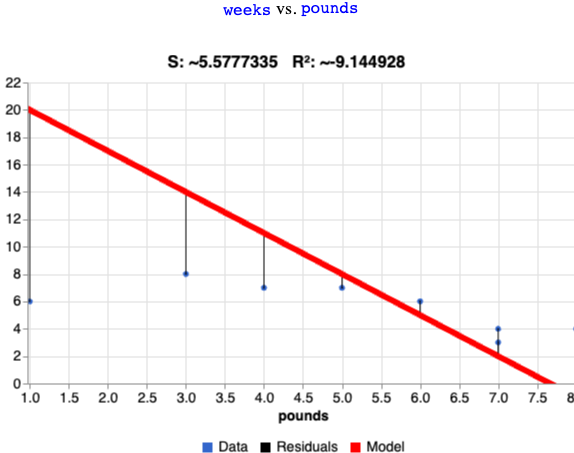
\includegraphics[width=0.48\textwidth]{images/6ea8d5a5bffc8a2f.png}\hfill
  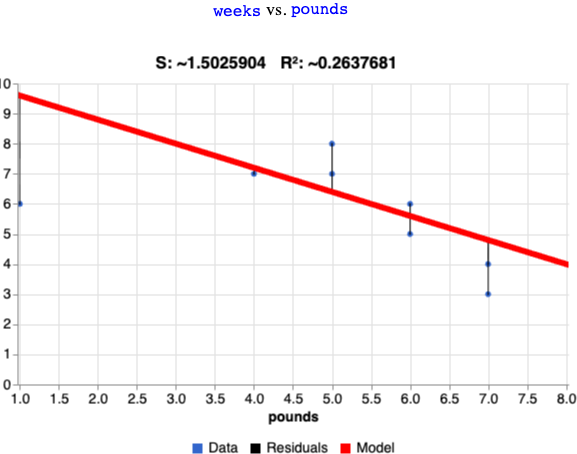
\includegraphics[width=0.48\textwidth]{images/3905e5489bec4b0a.png}
\end{center}
\begin{center}
\small\emph{Gauche~: ajustement du modèle de Cy ($S \approx 1{,}59$). Droite~: ajustement du modèle de Jo ($S \approx 5{,}91$).}
\end{center}

\begin{thinkbox}
  \begin{itemize}
    \item \textbf{Que remarquez-vous~?} Que vous demandez-vous~?
    \item \textbf{Comparez l'affichage de \texttt{fit-model} pour \texttt{cy} à celui de \texttt{jo}. En quoi sont-ils \emph{similaires}~? En quoi sont-ils \emph{différents}~?}
    \begin{itemize}
      \item Les deux modèles ont une ligne bleue et des points rouges.
      \item L'axe des $x$ va de 0 à 8 pour les deux.
      \item L'axe des $y$ pour \texttt{cy} est numéroté de 0 à 20. Il va de 3 à 9 pour \texttt{jo}.
      \item \texttt{jo} a plus de points rouges en dessous de la ligne bleue qu'au-dessus.
      \item Les points de données pour \texttt{jo} remplissent plus ou moins tout l'espace vertical de l'affichage, alors que pour \texttt{cy} il n'y a des points que dans la moitié inférieure.
    \end{itemize}
  \end{itemize}
\end{thinkbox}

\img{images/ece797adb2636c24.png}{width=0.5\textwidth}{Nuage de points avec droite de régression. Une ligne verticale est tracée entre le point prédit sur la droite et le point de données réel, pour montrer la taille du résidu en ce point.}

\begin{keypointbox}
  \textbf{Résidus}

  Quand nous traçons un modèle dans Pyret, nous pouvons voir que~:
  \begin{itemize}
    \item certains points sont proches de la ligne ($y$ «~réel~» proche de $y$ «~prédit~»)~;
    \item certains points sont assez loin ($y$ «~réel~» loin de $y$ «~prédit~»).
  \end{itemize}

  La différence entre tout $y$ réel et $y$ prédit est appelée le \textbf{résidu}, et mesure à quel point ce point du modèle s'écarte des données réelles. \emph{Plus les résidus sont petits, meilleur est l'ajustement~!}
\end{keypointbox}

\begin{thinkbox}
  \begin{itemize}
    \item \textbf{Il y a trois termes dans la légende en bas. À quoi se réfèrent-ils~?}
    \begin{itemize}
      \item La ligne bleue est le modèle.
      \item Les points rouges sont les données du jeu de données.
      \item Les résidus se réfèrent aux lignes noires verticales reliant les points de données au modèle, représentant la distance entre les données et la valeur prédite par le modèle. Ils varient en longueur selon la position du point au-dessus ou en dessous du modèle.
    \end{itemize}
  \end{itemize}
\end{thinkbox}

\begin{thinkbox}
  \begin{itemize}
    \item \textbf{Comment se comparent $S$ et $R^2$ pour les deux modèles~?}
    \begin{itemize}
      \item Les valeurs sont positives pour les deux modèles, et les valeurs de $S$ et $R^2$ sont toutes les deux plus petites pour \texttt{jo} que pour \texttt{cy}.
    \end{itemize}
    \item \textbf{Sur la base des valeurs de $S$ des graphiques que vous avez créés, que pensez-vous que $S$ signifie~?}
    \begin{itemize}
      \item Si un modèle a une valeur $S$ plus basse qu'un autre pour les mêmes données, cela indique un meilleur ajustement.
    \end{itemize}
  \end{itemize}
\end{thinkbox}

\begin{keypointbox}
  Tout comme il existe différents outils pour trouver le centre ou la dispersion d'un jeu de données, il y a de nombreux outils pour calculer la qualité d'ajustement d'un modèle, dont $S$ et $R^2$, que vous venez de voir en ajustant les modèles dans Pyret.

  Les statisticien·nes et data scientist·es veillent à utiliser le bon outil pour la bonne tâche~!
  \begin{itemize}
    \item Nous voulons une mesure qui prenne en compte les valeurs de \emph{chaque} point de données.
    \item Nous voulons une mesure d'\emph{erreur}, donc la mesure devrait être zéro pour un modèle parfaitement ajusté à chaque point (i.e.\ sans résidus).
    \item Nous voulons une mesure concrète et facile à comprendre.
  \end{itemize}
\end{keypointbox}

\begin{keypointbox}
  \textbf{La valeur~$S$}

  $S$ est une mesure de qualité d'ajustement, qui se réfère à l'\textbf{écart-type des résidus} (\emph{Standard Deviation of the Residuals}).

  \begin{itemize}
    \item Plus les points de données sont proches du modèle, plus les résidus sont petits.
    \item Dans un \emph{ajustement parfait}, $S$ serait~$0$.
    \item $S$ est exprimé en \emph{unités de la variable de réponse} (l'axe des $y$), ce qui la rend facile à interpréter.
    \begin{itemize}
      \item En ajustant un modèle à ce jeu de données, un $S$ de~5 signifie «~l'écart-type des résidus est de \textbf{5~semaines avant adoption}~».
    \end{itemize}
    \item En comparant deux modèles pour le \emph{même} jeu de données, le modèle avec le \emph{plus petit} $S$ est le meilleur~!
    \item Cela n'a pas de sens de comparer $S$ pour des modèles qui décrivent des jeux de données \emph{différents}.
  \end{itemize}

  \vspace{0.4em}
  \textbf{Vous ne pouvez pas calculer $S$ si vous n'avez que deux points de données~!} Nous utilisons deux points pour définir la ligne~; s'il ne reste aucune autre donnée, il n'y a rien à ajuster~! Pour calculer $S$, il faut une table avec \emph{trois points ou plus}.

  \vspace{0.4em}
  La valeur de $S$ doit toujours être considérée \textbf{dans le contexte de l'étendue} des valeurs prédites par le modèle~!
\end{keypointbox}

\subsection{Considérer \texorpdfstring{$S$}{S} dans son contexte}

\begin{activitybox}
  Considérez la valeur de $S$ de chaque modèle dans le contexte de l'étendue des données décrites. Décidez à quel point le modèle est susceptible de bien prédire les valeurs.

  \begin{enumerate}[leftmargin=*]
    \item Êtes-vous tout à fait d'accord pour dire qu'un des modèles décrit un bon ajustement~? Pourquoi~?
    \begin{itemize}
      \item Scénarios 2 et 8 — parce que les nombres dans l'étendue sont énormes et la valeur $S$ est très petite.
    \end{itemize}
    \item Êtes-vous tout à fait en désaccord pour dire qu'un des modèles est un bon ajustement~? Pourquoi~?
    \begin{itemize}
      \item Scénarios 1 et 6 — parce que la valeur $S$ est grande comparée à l'étendue.
      \item Pour le premier, $S = 300$, ce qui est la majorité de l'étendue entre 0 et 400.
      \item Pour le sixième, même si $S = 1$ seulement, c'est beaucoup plus grand que tous les nombres de l'étendue, qui vont jusqu'à deux centièmes.
    \end{itemize}
  \end{enumerate}
\end{activitybox}

\subsection{Expérimenter avec \texttt{fit-model} en direct}

\begin{activitybox}
  Maintenant que nous avons une idée de ce que fait \texttt{fit-model}, voyons-le fonctionner en direct dans Pyret~!

  \begin{itemize}
    \item Retournez au fichier \textbf{Échantillon de Lézards} (\texttt{Echantillon\allowbreak-Lezards\allowbreak-Starter.arr}).
    \begin{itemize}
      \item Remarquez que les fonctions \texttt{cy} et \texttt{jo} sont définies sur les lignes 26 et 28 de la Zone de Définitions.
      \item Juste après, vous verrez deux expressions \texttt{fit-model}~: l'une prend la fonction \texttt{cy}, l'autre \texttt{jo}.
    \end{itemize}
    \item Décommentez les deux dernières lignes de code et cliquez sur «~Run~».
  \end{itemize}

  \begin{enumerate}[leftmargin=*]
    \item Comment savons-nous que le premier graphique interactif qui apparaît ajuste le modèle de Cy aux données~?
    \begin{itemize}
      \item Parce que la première expression prend \texttt{cy} en argument.
    \end{itemize}
    \item Déplacez votre souris le long de la ligne. Quelles informations pouvons-nous tirer des fenêtres «~Modèle~»~?
    \begin{itemize}
      \item Les coordonnées de n'importe quel point du modèle.
    \end{itemize}
    \item Déplacez votre souris sur différents points et lisez les informations des fenêtres «~Données~». Que pouvons-nous apprendre~?
    \begin{itemize}
      \item Les coordonnées ($x$, $y$) de chaque point du jeu de données, et les animaux auxquels ils sont associés.
    \end{itemize}
    \item Trouvez la fenêtre «~Résidus~» en survolant l'un des points de données. Que pouvons-nous apprendre~?
    \begin{itemize}
      \item Les coordonnées ($x$, $y$) d'un point de données, la valeur prédite $\hat{y}$ pour ce $x$, et le «~résidu~»~: la différence entre $y$ et $\hat{y}$.
    \end{itemize}
    \item Que se passe-t-il une fois que nous fermons le deuxième graphique interactif~?
    \begin{itemize}
      \item Nous voyons des vignettes cliquables des deux graphiques dans la Zone d'Interactions.
    \end{itemize}
  \end{enumerate}
\end{activitybox}

\begin{instructornotes}
  \textbf{Optionnel~: Quel modèle est le meilleur~?}

  Si les élèves savent calculer l'équation d'une droite passant entre deux points, demandez-leur de définir leurs propres modèles pour \texttt{age} vs.\ \texttt{semaines} en Pyret et d'utiliser \texttt{fit-model} pour voir lequel est le meilleur.
\end{instructornotes}

\subsection{Interpréter nos modèles}

\begin{activitybox}
  Assurons-nous de connaître la signification des modèles que nous avons construits et des statistiques que nous avons recueillies à leur sujet.

  \begin{itemize}
    \item Complétez les deux premières sections de \emph{Interpréter nos modèles} avec votre voisin·e.
    \item \textbf{Attention~: vous allez utiliser les pourcentages de variation pour comparer les erreurs attendues de ces modèles.}
  \end{itemize}
\end{activitybox}

\begin{instructornotes}
  Les informations nécessaires à la première section se recueillent le plus facilement en regardant la table (dans Pyret) et en utilisant les fonctions \texttt{dot-plot} et \texttt{box-plot}.

  Confirmez que vos élèves peuvent compléter le modèle de Cy correctement. S'ils n'ont pas défini leurs propres modèles linéaires, demandez-leur d'ignorer la dernière section de la page.
\end{instructornotes}

\begin{thinkbox}
  \textbf{Comment $r^2$ peut-il être négatif~?}

  Les élèves attentifs pourraient se demander comment il est possible que $r^2$ soit négatif. C'est censé être impossible, non~?

  Il s'avère que le $R^2$ d'un modèle \emph{n'est pas} calculé en élevant $R$ au carré, et n'est effectivement égal à $R \times R$ que lorsque le modèle est produit par une \textbf{régression linéaire}. Rappelez-vous~: la régression linéaire ne peut trouver que la droite de \emph{meilleur} ajustement, donc elle ne produira jamais quelque chose d'aussi insensé qu'une ligne à pente négative pour un jeu de données à corrélation positive~!

  Quand les élèves créent leurs propres modèles, ne sont pas lié·es par l'algorithme de régression linéaire et peuvent proposer des droites dont l'ajustement est pire que tout ce que \texttt{lr-plot} pourrait produire~!
\end{thinkbox}

\subsection{Synthèse}

\begin{thinkbox}
  \begin{itemize}
    \item \textbf{Pourquoi devons-nous connaître l'étendue du jeu de données pour interpréter une valeur $S$~?}
    \begin{itemize}
      \item Les valeurs $S$ nous indiquent l'erreur attendue en \emph{unités de la variable sur l'axe des $y$}. Une erreur de 1000~€ peut être énorme ou minuscule selon le contexte.
    \end{itemize}
    \item \textbf{En plus de regarder la valeur $S$, que pourriez-vous chercher pour déterminer si un modèle linéaire est un bon ajustement pour les données~?}
    \begin{itemize}
      \item Que la distance moyenne des points au-dessus de la ligne semble à peu près la même que la distance moyenne des points en dessous de la ligne.
    \end{itemize}
  \end{itemize}
\end{thinkbox}

\begin{keypointbox}
  \emph{Tous les modèles se trompent. Certains sont utiles.}

  \begin{itemize}
    \item N'importe quelle ligne que nous tracerons sera-t-elle \textbf{parfaite}~? Pourquoi ou pourquoi pas~?
    \item Quand une ligne est-elle utile~?
  \end{itemize}
\end{keypointbox}

\newpage

% ===========================================================================
% ANNEXES
% ===========================================================================
\section*{Annexe A~: Schéma d'un résidu}

La figure ci-dessous montre comment un résidu est mesuré~: pour chaque point de données $(x_i, y_i)$, on trace une ligne verticale entre le point réel et la valeur prédite $\hat{y}_i = f(x_i)$ sur le modèle. La longueur de cette ligne verticale est le résidu~: $e_i = y_i - \hat{y}_i$.

\begin{center}
\begin{tikzpicture}[>=Stealth, scale=1.1]
  % Axes
  \draw[->, thick] (0,0) -- (6.5,0) node[right] {$x$ (poids)};
  \draw[->, thick] (0,0) -- (0,4.5) node[above] {$y$ (semaines)};
  % Régression line
  \draw[modelline, very thick] (0.2,4.2) -- (6.2,0.8) node[right, text=black, font=\small] {modèle $f$};
  % Data points + residuals
  \foreach \x/\y in {1/3.5, 2/3.8, 3/2.6, 4/2.2, 5/1.5} {
    \fill[datadot] (\x,\y) circle (3pt);
    \pgfmathsetmacro{\yhat}{4.2 - 0.567*\x}
    \draw[dashed, thick, black!70] (\x,\y) -- (\x,\yhat);
  }
  % Annotated residual
  \draw[<->, thick, bsorange] (3,2.6) -- (3, 2.5) node[midway, right, font=\scriptsize\bfseries, text=bsorange] {résidu};
  % Legend
  \node[anchor=west, font=\small] at (4.5, 4) {\textcolor{datadot}{$\bullet$} données};
  \node[anchor=west, font=\small] at (4.5, 3.6) {\textcolor{modelline}{\textbf{---}} modèle};
  \node[anchor=west, font=\small] at (4.5, 3.2) {\textcolor{bsorange}{\textbf{|}} résidu};
\end{tikzpicture}
\end{center}

\begin{center}
  
\includegraphics[width=0.5\textwidth]{images/ece797adb2636c24.png}
\end{center}
\begin{center}
\small\emph{Vue Pyret correspondante~: à chaque point rouge, une ligne verticale noire montre la distance entre les données réelles et la prédiction du modèle.}
\end{center}

\section*{Annexe B~: Exercices supplémentaires}

\begin{itemize}
  \item L'activité Desmos \emph{Fit Fights} (inspirée par Illustrative Mathematics et OpenUp Resources) demande aux élèves de placer une droite sur un nuage de points en essayant de maximiser un compteur mesurant la qualité de l'ajustement. Recommandée comme pratique supplémentaire à la maison ou comme activité d'ouverture après cette leçon.
  \item Pour davantage de pratique~: \emph{Comment pourrions-nous mesurer si un modèle est un bon ajustement~? (Cheerios)}, avec le \emph{Cheerios Starter File} de Bootstrap~:
  \begin{lstlisting}
fit-model(cheerios-table, "id", "day", "cheerios-on-the-floor", f)
fit-model(cheerios-table, "id", "day", "cheerios-on-the-floor", g)
  \end{lstlisting}
\end{itemize}

\begin{center}
  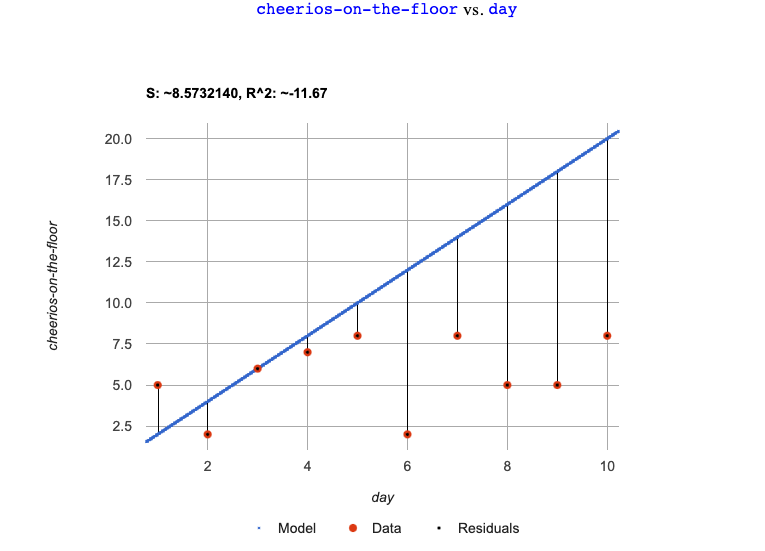
\includegraphics[width=0.48\textwidth]{images/a8c1616af8a3b27c.png}\hfill
  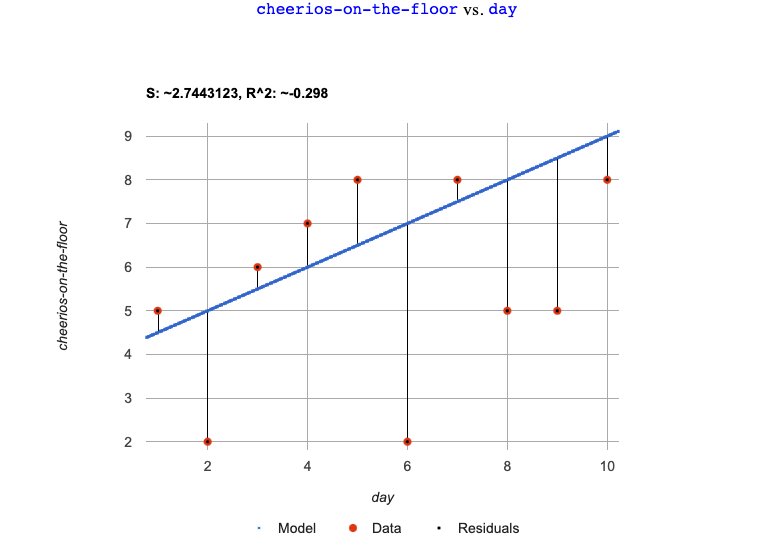
\includegraphics[width=0.48\textwidth]{images/190a74cf424d3f3e.png}
\end{center}
\begin{center}
\small\emph{Ajustement des modèles $f$ et $g$ sur le jeu de données Cheerios, avec affichage des résidus.}
\end{center}

\section*{Annexe C~: Fichiers du projet}

\begin{center}
\begin{tabularx}{\textwidth}{l X}
  \toprule
  \textbf{Fichier} & \textbf{Description} \\
  \midrule
  \texttt{Echantillon\allowbreak-Lezards\allowbreak-Starter.arr} & Fichier de démarrage Pyret~: charge \texttt{core.arr} depuis Bootstrap + CSV français depuis GitHub. Définit \texttt{lizard-sample}, \texttt{cy}, \texttt{jo}. \\
  \texttt{ajuster-modeles.tex} & Document de cours (ce fichier) \\
  \texttt{dictionaries/lizard-sample-fr.csv} & 10 lézards (colonnes~: \texttt{nom, espece, sexe, age, sterilise, pattes, poids, semaines}) \\
  \texttt{images/} & Nuages de points, modèles ajustés, schéma de résidu, photos de lézards (8 PNG) \\
  \bottomrule
\end{tabularx}
\end{center}

\vspace{1em}
\textbf{À noter~:} contrairement à l'original anglais qui utilise \texttt{load-spreadsheet} pour charger les données depuis Google Sheets, notre adaptation française charge le CSV depuis le dépôt GitHub du projet via \texttt{csv.csv-table-url}. Aucune dépendance Google n'est requise. La bibliothèque \texttt{core.arr} de Bootstrap (qui fournit \texttt{scatter-plot}, \texttt{fit-model}, \texttt{dot-plot}, \texttt{box-plot}) est chargée via \texttt{use context url-file(...)} comme dans l'original.

\section*{Annexe D~: Pour aller plus loin}

\begin{instructornotes}
  \textbf{Et les modèles non linéaires~?}

  Rien n'oblige à s'arrêter à la droite de meilleur ajustement~! Les enseignant·es de mathématiques avancées (ou les enseignant·es de Sciences des Données qui souhaitent compter leur cours comme alternative au programme avancé) peuvent étendre ce travail de modélisation avec les supports \emph{Algebra~2} de Bootstrap, qui couvrent les modèles quadratiques, exponentiels, logarithmiques et périodiques~!
\end{instructornotes}

\section*{À propos de ces supports}

Ces supports ont été développés en partie grâce au soutien de la \emph{National Science Foundation} (bourses 1042210, 1535276, 1648684, 1738598, 2031479 et 1501927).

\begin{center}
  \textbf{Bootstrap} par la Communauté Bootstrap est sous licence Creative Commons 4.0 Unported.\\
  Cette licence n'accorde pas la permission d'organiser des formations ou du développement professionnel.\\[1em]
  \textit{Traduction et adaptation française réalisées en juillet 2026.}\\
  \textit{Source originale~: \url{https://www.bootstrapworld.org/materials/fall2026/en-us/lessons/fitting-models/}}
\end{center}

\end{document}